\documentclass{article}
\usepackage{graphicx} % Required for inserting images
\usepackage{amsmath}
\usepackage{amssymb}

\usepackage{tikz}
\usetikzlibrary{positioning}
\usetikzlibrary{calc}


\title{Deriving Backpropagation Gradients}
\author{Amelia}
\date{February 2026}

\begin{document}

\maketitle
\section{Deriving the gradients for a single value}
Let us derive the gradients that happen in backpropogation, one value at a time.

$$\text{let }\theta, W\in \mathbb R^n \text{ and } n \text{ be an arbitrary value}$$

\begin{figure}[!h]
\centering
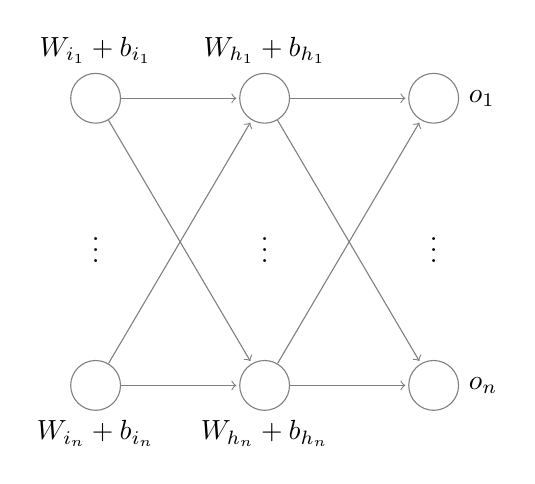
\begin{tikzpicture}[
    shorten >=1pt,
    ->,
    draw=black!50,
    node distance=3cm and 1.5cm
]
\tikzstyle{unit}=[circle, draw, minimum size=18pt, inner sep=0pt]

% Input layer
\node[unit] (i1) {};
\node[unit, below=of i1] (in) {};
\node at ($(i1)!0.5!(in)$) {$\vdots$};
\node[above] at (i1.north) {$W_{i_1}+b_{i_1}$};
\node[below] at (in.south) {$W_{i_n}+b_{i_n}$};

% Hidden layer
\node[unit, right=of i1] (h1) {};
\node[unit, below=of h1] (hn) {};
\node at ($(h1)!0.5!(hn)$) {$\vdots$};
\node[above] at (h1.north) {$W_{h_1}+b_{h_1}$};
\node[below] at (hn.south) {$W_{h_n}+b_{h_n}$};

% Output layer
\node[unit, right=of h1, label=right:$o_1$] (o1) {};
\node[unit, below=of o1, label=right:$o_n$] (on) {};
\node at ($(o1)!0.5!(on)$) {$\vdots$};

% Connections
\draw (i1) -- (h1);
\draw (i1) -- (hn);
\draw (in) -- (h1);
\draw (in) -- (hn);

\draw (h1) -- (o1);
\draw (h1) -- (on);
\draw (hn) -- (o1);
\draw (hn) -- (on);

\end{tikzpicture}

    \caption{A typical Neural Net}
    \label{fig:1}
\end{figure}

\begin{align}
W_{h_1} &\leftarrow W_{h_1} - \alpha \left( \frac{\partial o_1}{\partial W_{h_1}} + \dots + \frac{\partial o_n}{\partial W_{h_1}} \right) \\
b_{h_1} &\leftarrow b_{h_1} - \alpha \left( \frac{\partial o_1}{\partial b_{h_1}} + \dots + \frac{\partial o_n}{\partial b_{h_1}} \right)
\end{align}

\section{Deriving gradients in the vector case}
\begin{gather}
    W_h \doteq 
    \begin{pmatrix}
        W_{h1} \\
        W_{hn}
    \end{pmatrix}
    \quad
    b_h \doteq 
    \begin{pmatrix}
        b_{h1} \\
        b_{hn}
    \end{pmatrix}
    \quad
    O_h \doteq 
    \begin{pmatrix}
        o_{h1} \\
        o_{hn}
    \end{pmatrix}
\end{gather}

\begin{align}
\frac{\partial o}{\partial W_h} &\doteq \begin{pmatrix}
\frac{\partial o}{\partial W_{h_1}} \\
\vdots \\
\frac{\partial o}{\partial W_{h_n}}
\end{pmatrix} \\
&= \begin{pmatrix}
\frac{\partial o_1}{\partial W_{h_1}} + \dots + \frac{\partial o_n}{\partial W_{h_1}} \\
\vdots \\
\frac{\partial o_1}{\partial W_{h_n}} + \dots + \frac{\partial o_n}{\partial W_{h_n}}
\end{pmatrix}
\end{align}

\section{Deriving gradients in earlier layers}

We are trying to find $\frac{\partial o}{\partial W_i}$. Through the chain rule, we can expand this into:

$$\frac{\partial o}{\partial W_i} = \frac{\partial o}{\partial W_h}\frac{\partial W_h}{\partial W_i}$$


\end{document}
